\documentclass{article}
\usepackage{graphicx}

\title{C\# Reverse Engineering}


\begin{document}
\maketitle

\section*{C\# Compilation Process}
C\# $\to$ CIL $\to$ machine code

CIL (MSIL) is the code that is distributed among users (.exe and stuff). Is compiler by CLR to machine code


\begin{figure}[h]
    \centering
    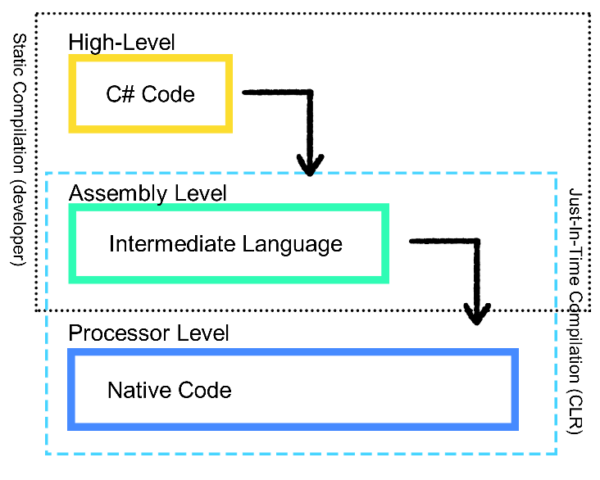
\includegraphics[width=10cm]{how-is-c-compiled_01-600x480.png}
    \caption{TBD}
    \label{fig:TBD}
    % https://freecontent.manning.com/how-is-c-compiled/
\end{figure}

Thus, for static reverse engineering we can use a CIL decompiler

\section*{CIL Decompilers}

Since the compiler embeds CIL in executable files, we need to use a disassembler to view the CIL. All .NET flavors come with such a tool called IL DASM (which stands for Intermediate Language Disassembler). To use IL DASM, we need to run the “Developer Command Prompt for Visual Studio” which is installed alongside Visual Studio. This is a command prompt environment that gives us access to .NET tools. Be aware that IL DASM is only available for Windows.
% https://freecontent.manning.com/how-is-c-compiled/

monodis to decompile machine code to CIL

ILSpy NuGet decompiles to C# (Whole-project decompilation (csproj, not sln!)) 
% https://github.com/icsharpcode/ILSpy

https://docs.microsoft.com/en-us/archive/msdn-magazine/2003/november/thwart-reverse-engineering-of-your-visual-basic-net-or-csharp-code

\section*{Side Notes}

Intermediate Language can easily be decompiled (whether originally compiled in debug or release mode) to something similar to the original source code. If you want to appropriately protect your source code, consider looking into obfuscators (Dotfuscator, NET Reactor) and threat models. 
% https://freecontent.manning.com/how-is-c-compiled/

\end{document}